%% Dummy intro.tex.
%% Not under the license, just here to ensure the template compiles properly.
%% Also contains a couple of examples.

\chapter{Introduction}\label{ch:intro}

\section{Examples}

\lipsum[1-2]

\begin{equation} \label{eq:heart-eq}
  F\left\{ \heartsuit \right \} =
  \frac{1}{\sqrt{2\pi}} \int\limits_{-\infty}^{\infty} f(t) e^{i t \heartsuit} \mathrm{d} t
  = \text{\textbf{?}}
\end{equation}

Equation (\ref{eq:heart-eq}) shows us that this is still an unsolved problem.

\lipsum[3]

\begin{figure}
  \centering
  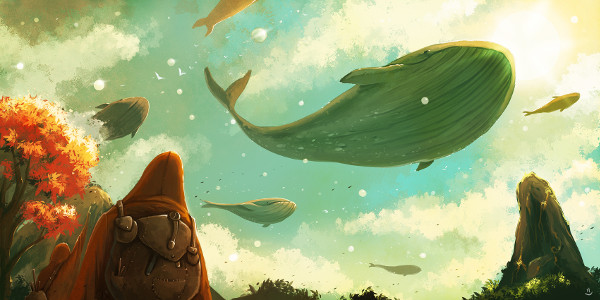
\includegraphics[width=0.8\linewidth]{the-ocean-sky}
  \caption[The Ocean Sky]{The Ocean Sky by Desmond Wong, licensed under a
    \emph{Creative Commons Attribution-NonCommercial 3.0 Unported License}.}
  \label{fig:ocean-sky}
\end{figure}

Figure \ref{fig:ocean-sky} is the same figure as the front page figure. The
difference is that we use it to give an example on how to center and include it
as a figure.

\lipsum[4]

Citation of the C11 standard\cite{iso2011c}.

\lipsum[11-12]

\begin{listing}
  \inputminted[frame=single,linenos,fontsize=\small,mathescape]{scm}{lst/sqrt-iter.scm}
  \caption[Square Roots in Scheme]{Implementation of Square Roots by Newton's
    Method in Scheme, from SICP.}
  \label{lst:sqrt-iter}
\end{listing}

Listing \ref{lst:sqrt-iter} shows us how code blocks will look like. Change the
colours palette inside \texttt{config.tex} if you want another one.

\lipsum[13]
